%!TEX root = ./main.tex
\section{Implementation}
\label{sec:implementation}




\begin{figure}[t]
	\centering
	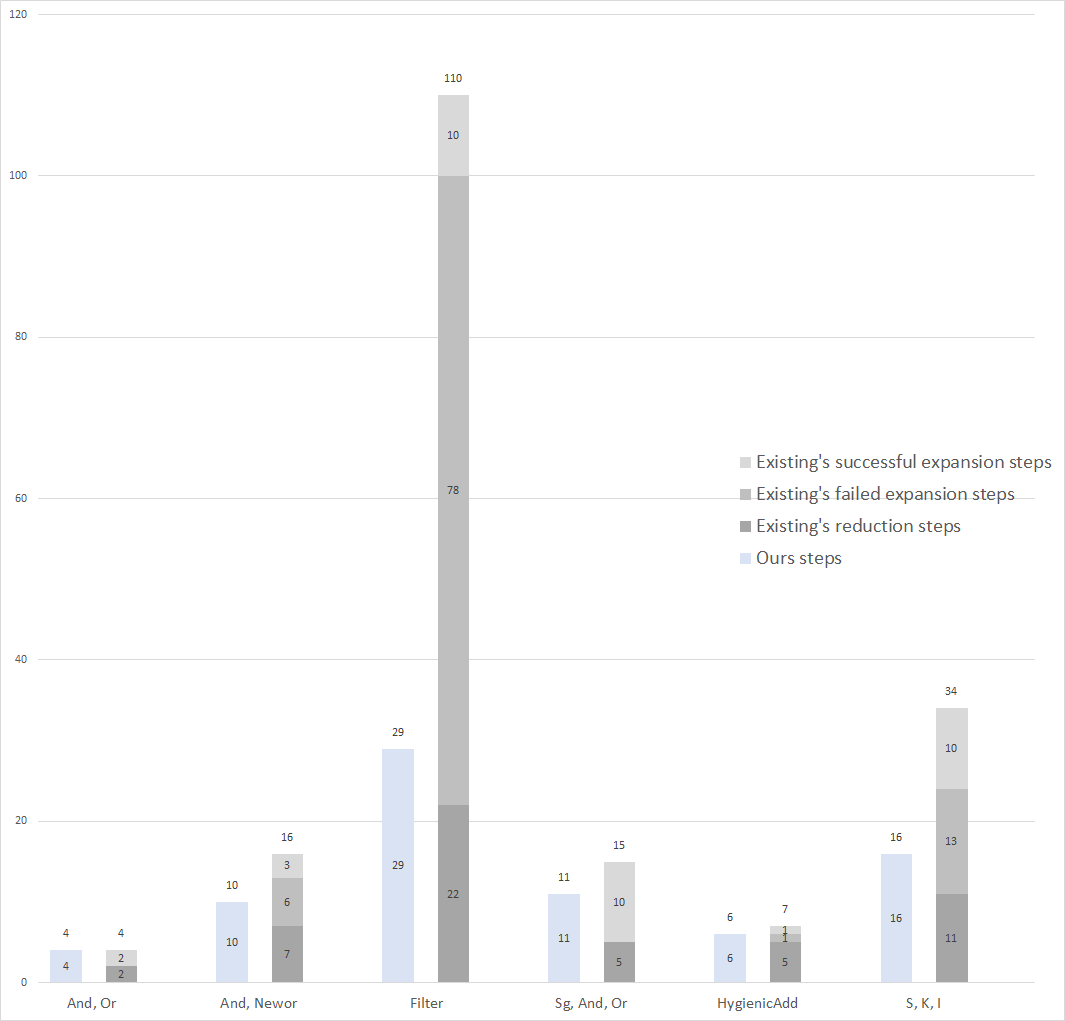
\includegraphics[width=0.6\textwidth]{images/efficiency.png}
	\caption{Comparison on Reduction Steps}
	\label{fig:step}
\end{figure}
We have implemented our resugaring approach using PLT Redex \cite{SEwPR}, a semantic engineering tool based on reduction semantics \cite{reduction}. We also test the efficiency with some examples.

To show the efficiency of our approach, we use the number of reduction steps comparing to the existing approach as the metrics. Figure \ref{fig:step} shows the difference between the two approaches. Notice that both approaches have some preprocessing---for the existing one, it is to desugar the programs to the core language together with some tags; for ours, it is to calculate the context rules of syntactic sugars. We do not consider the steps during preprocessing. Besides, we derive the reduction steps of the existing approach into three different kinds---the reductions in the core language, the reverse expansion with failed resugaring, the reverse expansion with successful resugaring.  Use the following example to see the difference. Consider a sugar named \m{Hard} with two arguments, which has many reduction steps after desugared. Assuming for specific $e_1$ and $e_2$, the \Code{(Hard $e_1$ $e_2$)} after fully desugared has 100 reduction steps (e.g. finally to \m{\false}), and only 1 intermediate step ($\m{step}_n$) can be resugared (e.g. to \Code{(Hard $v_1$ $e_2$)}). Then for \Code{(And (Hard $e_1$ $e_2$) \#t)}, although all the 100 steps in the core language try the reverse desugaring, only \Code{(if $\m{step}_n$ \#t \#f)} (2 steps on \m{And}, \m{Hard}) and \Code{(if \#f \#t \#f)} (1 step on \m{And}) are successful. Other 98 attempts will be failed with 98 failed reverse expansion steps on \m{And}.

\[
{\footnotesize
	\begin{array}{lcl}
	\text{Surface}&&\text{Core}\\
	\Code{(And (Hard $e_1$ $e_2$) \#t)}&\xrightarrow{desugar}&\Code{(if $\m{step}_0$ \#t \#f)}\\
	\qquad\quad\dashdownarrow& &\qquad\qquad\downarrow\\
	\Code{(And $\m{step}_1$ \#t)}&\xleftarrow{resugar}&\Code{(if $\m{step}_1$ \#t \#f)}\\
	\qquad\quad\vdots& &\qquad\qquad\vdots\\
	\Code{(And (Hard $v_1$ $e_2$) \#t)}&\xleftarrow{resugar}&\Code{(if $\m{step}_n$ \#t \#f)}\\
	\qquad\quad\vdots& &\qquad\qquad\vdots\\
	\Code{(And \#f \#t)}&\xleftarrow{resugar}& \Code{(if \#f \#t \#f)}\\
	\qquad\quad\dashdownarrow& &\qquad\qquad\downarrow\\
	\Code{\#f}&& \Code{\#f}\\
\end{array}
}
\]


The general tendency is---the more complex the sugar is, the more steps will our approach save. Note that if the RHS of a syntactic sugar is huge, a one-step reduction of the reverse desugaring will also be complex, because huge sugars will contain many failed attempts to resugar. So avoiding reverse expansion of syntactic sugar can improve the efficiency for practical use because programs are usually not that small like the demos.
